% \subsubsection{Caughey}
% ** Not in  release ** The model  is a particular case of  the Rayleigh damping
% model,   with    damping   being   proportional   only    to   the   stiffness
% matrix. Substitute with complete Rayleigh damping model for release?

\subsubsection{Neo-Hookean}\index{Material!Neohookean}

The Neo-Hookean constitutive law is a hyperelastic material formulation, which
results from an extension of the linear elastic relationship (Hooke's Law) for
large deformation. Thus, the model predicts nonlinear stress-strain behavior for
bodies undergoing large deformations.

\begin{figure}[!htb]
  \begin{center}
    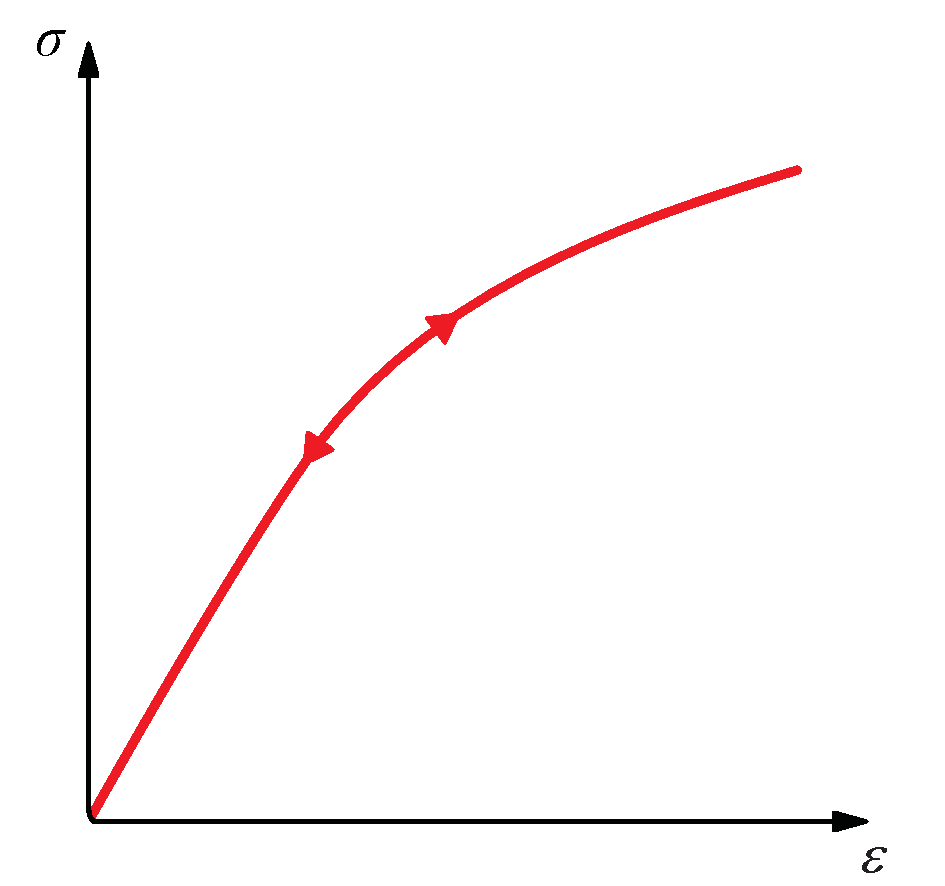
\includegraphics[width=0.4\textwidth,keepaspectratio=true]{figures/stress_strain_neo.pdf}
    \caption{Neo-hookean Stress-strain curve.}
    \label{fig:smm:cl:neo_hookean}
  \end{center}
\end{figure}

As illustrated in Figure~\ref{fig:smm:cl:neo_hookean}, the behavior is initially
linear and the mechanical behavior is very close to the corresponding linear
elastic material. This constitutive relationship, which accounts for compressibility,
 is a modified version of the one proposed by Ronald Rivlin \cite{Belytschko:2000}.

The strain energy stored in the material is given by:
\begin{equation}\label{eqn:smm:constitutive:neohookean_potential}
  \Psi(\mat{C}) = \frac{1}{2}\lambda_0\left(\ln J\right)^2-\mu_0\ln J+\frac{1}{2}
\mu_0\left(\text{trace}(\mat{C})-3\right)
\end{equation}
\noindent where $\lambda_0$ and $\mu_0$ are, respectively, the Lam\'e's first parameter
and the shear modulus at the initial configuration. $J$ is the jacobian of the deformation
gradient ($\mat{F}=\nabla_{\!\!\vec{X}}\vec{x}$): $J=\text{det}(\mat{F})$. Finally $\mat{C}$ is the right Cauchy-Green
deformation tensor.

Since this kind of materials is used for problem involving large deformations, a finite
deformation framework should be used. Therefore, the Cauchy stress ($\mat{\sigma}$) should
be computed through the second Piola-Kirchhoff stress tensor $\mat{S}$:

\begin{equation}
  \mat{\sigma } = \frac{1}{J}\mat{F}\mat{S}\mat{F}^T
\end{equation}

Finally the second Piola-Kirchhoff stress tensor is given by:

\begin{equation}
  \mat{S}  = 2\frac{\partial\Psi}{\partial\mat{C}} = \lambda_0\ln J 
\mat{C}^{-1}+\mu_0\left(\mat{I}-\mat{C}^{-1}\right)
\end{equation}

The parameters to indicate in the material file are the same
as those for the elastic case: \code{E} (Young's modulus), \code{nu} (Poisson's
ratio).

\subsubsection{Visco-elastic (IMPLEMENTATION TO VERIFY!!)}

% Standard Solid rheological model, see [] J.C. Simo, T.J.R. Hughes,
% "Computational Inelasticity", Springer (1998), see Sections 10.2 and 10.3
Visco-elasticity is characterized by time dependent strain behavior. Moreover,
when such a material undergoes a deformation it dissipates some energy. This
dissipation results in a hysteresis loop in the stress-strain curve at every
loading cycle (see Figure~\ref{fig:smm:cl:visco-elastic:hyst}). In principle, it
can be applied to many materials, since all materials exhibit a visco-elastic
behavior if subjected to particular conditions (such as high temperatures).
\begin{figure}[!htb]
  \begin{center}

    \subfloat[]{
      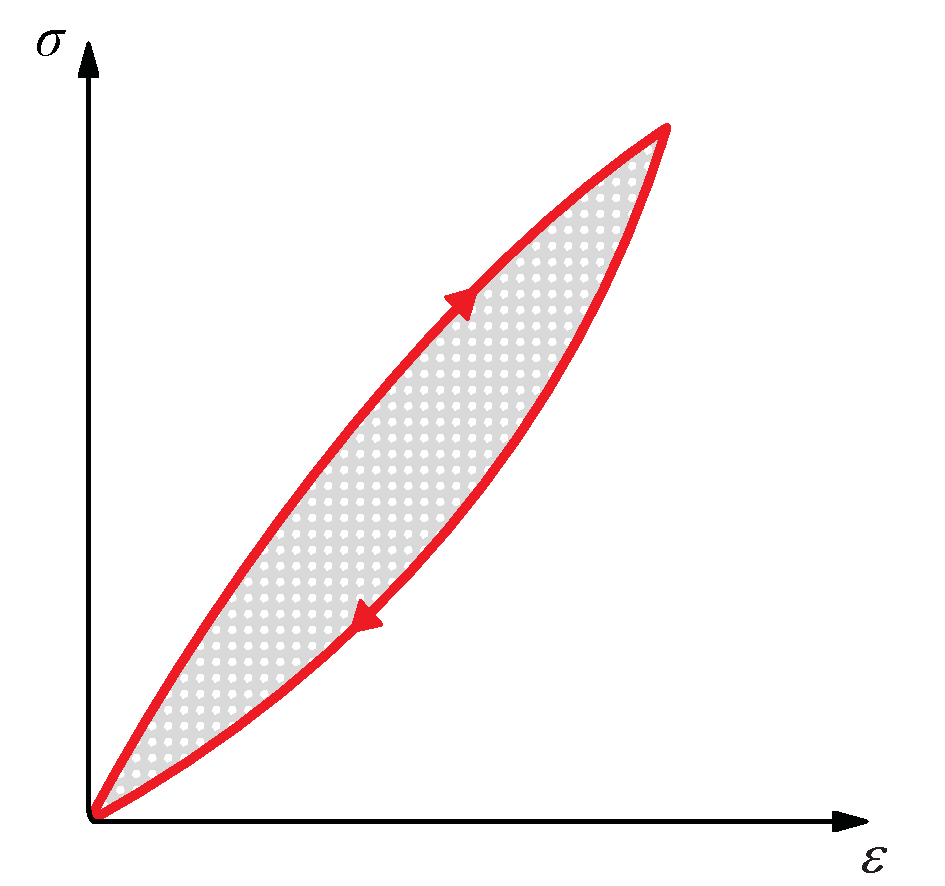
\includegraphics[width=0.4\textwidth,keepaspectratio=true]{figures/stress_strain_visco.pdf}
      \label{fig:smm:cl:visco-elastic:hyst}
    }
    \hspace{0.05\textwidth}
    \subfloat[]{
      \raisebox{0.025\textwidth}{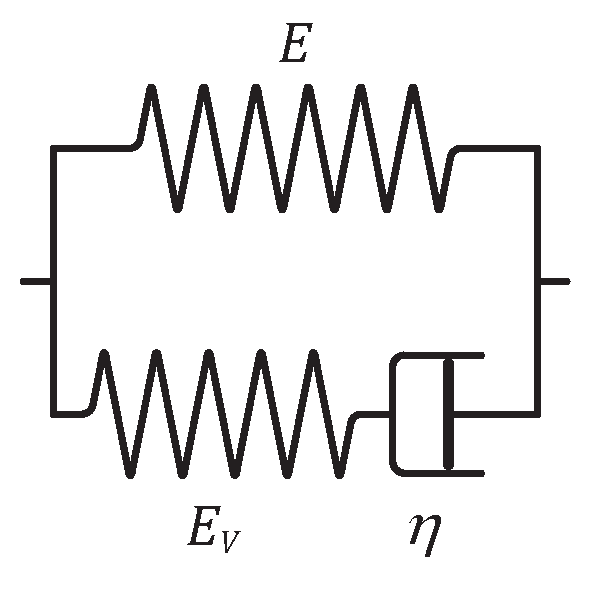
\includegraphics[width=0.3\textwidth,keepaspectratio=true]{figures/visco_elastic_law.pdf}}
      \label{fig:smm:cl:visco-elastic:model}
    }
    \caption{(a) Characteristic stress-strain behavior of a visco-elastic material with hysteresis loop and (b) schematic representation of the standard rheological linear solid visco-elastic model.}
    \label{fig:smm:cl:visco-elastic}
  \end{center}
\end{figure}
The standard rheological linear solid model (see Sections 10.2 and 10.3
of~\cite{simo92}) has been implemented in \akantu. This model results from the
combination of a spring mounted in parallel with a spring and a dashpot
connected in series, as illustrated in
Figure~\ref{fig:smm:cl:visco-elastic:model}. The advantage of this model is that
it allows to account for creep and stress relaxation. The equation that relates
the stress to the strain is (in 1D):
\begin{equation}
  \frac{d\epsilon(t)}{dt} = \left ( E + E_V \right ) ^ {-1} \cdot \left [ \frac{d\sigma(t)}{dt} + \frac{E_V}{\eta}\sigma(t) - \frac{EE_V}{\eta}\epsilon(t) \right ]
\end{equation}
where $\eta$ is the viscosity. The equilibrium condition is unique and is
attained in the limit, as $t \to \infty $. At this stage, the response is
elastic and depends on the Young's modulus $E$.  The parameters requested in the
material file are the following: \code{rho} (density), \code{E} (Young's
modulus), \code{nu} (Poisson's ratio), \code{Plane\_Stress} (if set to zero
plane strain, otherwise plane stress), \code{eta} (dashpot viscosity) and
\code{Ev} (stiffness of the viscous element).

\subsubsection{Damage Marigo}
\subsubsection{Damage Mazars}
